\documentclass{acm_proc_article-sp}
\usepackage{enumerate}
\usepackage{url}
\usepackage{listings}
\begin{document}

\title{Applying {\ttlit Mutation Sensitivity Testing} Techniques on Current Scientific Software}

\numberofauthors{2} 
\author{
% 1st. author
\alignauthor
Hussein Mosleh\\
       \affaddr{King Abdullah University of Science and Technology}\\
       \affaddr{H. 4106}\\
       \affaddr{Thuwal Saudi Arabia}\\
       \email{hussein.mosleh@kaust.edu.sa}
% 2nd. author
\alignauthor
Abdurrahman Abdulmoneim\\
       \affaddr{King Abdullah University of Science and Technology}\\
       \affaddr{H. 4106}\\
       \affaddr{Thuwal Saudi Arabia}\\
       \email{abdurrahman.abdulmoneim@kaust.edu.sa}
}

\maketitle
\begin{abstract}
Having a fault in a scientific software code is one of the most annoying problems a scientist may face. Scientific Software Engineers have come up with some useful tools and ways in order to solve such a problem. However, most of these methods or techniques have some issues that make them difficult for many scientists to adopt and use. One of such problems is requiring large number of tests for the scientific software which will waste time and effort.

In our project we used a technique that solves these problems and is very effective in assessing test cases of scientific software. This technique is called Mutation Sensitivity Testing which is an improved version of the traditional Mutation Testing. We applied this technique on an open source code and improved it in a sense that makes it more powerful.
\end{abstract}

%A category including the fourth, optional field follows...
\category{D.2.5}{Software Engineering}{Testing and Debugging}

\terms{Testing}

\keywords{Scientific software engineering, Mutation testing} % NOT required for Proceedings

\section{Introduction}

Software engineering is a mature field. It has a history of decades in the development of methods and processes for the creating and testing of software. Software engineering has attempted to construct processes and methods that are general enough to be used in any field that depends on computer software.

Computational scientists have stood out as a group that is least ready to adopt the processes developed by software engineers. It seems that there is a great gap between the two fields that prevents them from useful collaboration, and to even harshly criticize each other's methodologies. The reason for this lack of collaboration is that computational scientists have specialized needs stemming from the nature of their work. 

Since computational scientists have virtually no ``correct outputs'' to test against, they are more concerned with accurate rather than correct results. Also, computational scientists seem to be more concerned with trying new methods and showing outputs without attempting to question their products. Software engineers on the other hand have created solutions that are too general to be of value to them.\cite{a3}

Software engineering also does not provide methods that address the needs of computational scientists; such as the choice of test data or test cases set, long run time and huge data. This work attempts to bridge the gap between these tow disciplines by applying a testing method that is rooted in the practices of software engineering while being of practical value to the computational scientists community; The Mutation Sensitivity Testing (MST). The exact job for such technique is to test the reliability of the tests provided for almost any scientific code.\cite{a2}

\section{Motivation}
Faulty code in any scientific software may cause severe effects in its result's accuracy and wastes a lot of time and effort in order to figure out the fault.

Paul Dubois, a scientist, writes ``Small programming mistakes can be indistinguishable from incorrect modelling. I have spent hours in meetings looking for errors with scientists who speculated about whether some new piece of physics must be added in order to obtain a better answer. A week later, I learn that they had found a simple error [i.e., a code fault], and there was no scientific problem after all'' \cite{a4}.

This is one of the situations that encourages us to find a systematic and powerful software engineering method to help in testing and then catching any fault in given scientific software.

There are two factors that lead to the difficulty of testing any scientific software. The first factor is the limitation of comparing software outputs to expected results. The second factor is the large number of tests required when following any standard testing technique that exists in the software engineering publications\cite{a2}.

Mutation sensitivity testing, which we apply here in this project, tries to tackle these challenges. It proves that a small number of well-designed tests can detect many code faults. It does that by making sure that your test cases are enough to find any fault that may occur in your original code. Furthermore, it shows that reducing error tolerances is often far better than running large number of tests. Figure 1 shows possible sources of faults in scientific software.

\begin{figure}[h]
\caption{possible sources of faults in scientific software \cite{a2}}
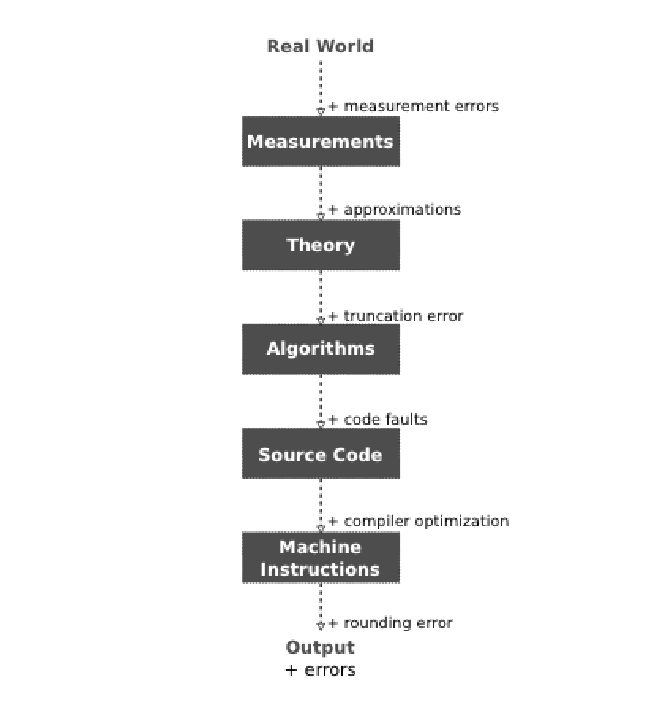
\includegraphics[scale=0.55]{fig1.png}
\end{figure}

\section{Background}


Mutation Testing is a software engineering tool which tests the test cases of a given software. This method does so by injecting defects in to the original code and then checking whether the test cases can detect these defects or not.

Mutation sensitivity testing is a modification to classical mutation testing methods. In the classical method, a set of ``mutations'' is defined. These mutations when applied to a source file will produce new source files (Mutants) that are faulty versions of the original one. A mutation could be, for example, changing an occurrence of `$<$' to `$>$'.

After generating the set of mutants, each mutant is run against the set of test cases, and their results are compared against the original code result. The mutants that produce a different output from the original are named ``dead mutants'' and discarded. Other mutants are called ``Survivors''.Those survivors are analysed to produce test cases that can ``kill'' them.

Mutation sensitivity testing builds upon this idea [3]. Instead of comparing the exact outputs, the test calculates the ``sensitivity'' of each mutant; a more relaxed measure, and attempts to kill mutants with low sensitivity. In this work, we attempt to build upon the work of Hook [2] in mutation sensitivity testing.

We can summarize the methodology of the mutation testing as follows:
\begin{enumerate}

\item Mutants Generation:
Mutants are faulty versions of the original tested code. These can be generated by one of the following ways:

\begin{enumerate}[i)]
\item Statement/block Deletion: like deleting an IF block or a WHILE loop or a simple addition statement from the original code.
\item Conditional Negation in IF and While structures.
\item Constant Replacement e.g. C+1, C-1, 0.9*C, 0*C where C is a constant in the original code.
\item Operator Replacement:
\begin{enumerate}[a)]
\item Mathematical Operators: $- , + , \div, \times$.
\item Comparison Operators : $<, >, =, \leq, \geq $.
\item Boolean operators : $\wedge, \vee$. 
\end{enumerate}

\end{enumerate}

\item Running and Evaluation:
Here we run the test cases set in each of the mutants and then evaluate their results by one of the evaluation methods (traditional, relative sensitivity or absolute sensitivity). We classify these mutants accordingly to two sets :
\begin{enumerate}[i)]
\item Survivors mutants: which has correct results as the original code. 
\item Dead mutants: which got erroneous results.
\end{enumerate}

\item Ignoring the identical survivors to the original code.

\item Percentage of test cases reliability depending on how many survivors we end up with. The fewer survivors the better percentage. 

\end{enumerate}

\section{Our work}

In addition to implementing the Mutation Sensitivity Testing that was invented in 2009 \cite{a2}, we added some other important enhancements:
\subsection{Python Framework}

We chose Python since it is widely used in the scientific computing world in general which we is our target. Python is also a powerful object oriented language that can be used in a wide range of software domains since it has a considerable amount of libraries and defined functions that can ease the software implementation.

In addition to that, Python is an interactive language which is used the same way as the Linux command line. A statement is entered, followed by the Enter key and the result then is printed on your screen. This is very helpful in debugging the code. Furthermore, this way is the natural way that is used in many mathematical programming used in the science such as Mathematica, and Matlab.\cite{a1}

Python also is a portable language. The Python interpreter can be installed on any architecture that has a C compiler. Because it is an interpreted language, programs that are written on one architecture can run on another. Also, you can have Python for free. Releases on all platforms are available for free which makes it easier to get.

\subsection{Traditional, Absolute Sensitivity and Relative Sensitivity Testing}
Our framework offers to the user to choose the type of Mutation Testing. We have implemented three types of testing that will suite most of the scientific software needs. The three types are:

\begin{enumerate}
\item Traditional Mutation Testing:

This kind of mutation testing appeared in the seventies. It actually strictly compares the equality of the output of the original code $P_0$ and the output of each of the generated mutants. Although this test is used very frequently but it is not that useful for most of the scientific computing \cite{a2}.

\item Relative Sensitivity Mutation Testing:

This type of Mutation testing was invented recently, namely in 2009 \cite{a2}. It was developed to solve the problem of the strict equality comparison done in the traditional way. It actually gives some sort of relative tolerance when evaluating the generated mutants' output. The relative tolerance can be given in this formula \cite{a2}:\\

\begin{center}
$\gamma(P_m, t) = \frac{|P_m(t) ? P_0(t)|}{|P0 (t)|}$
\end{center}

Here $\gamma(P_m,t)$ is the relative error for a given mutation $P_m$. $P_0(t)$ is the output of the original code. Our framework gives the scientist the freedom to choose the value of the relative tolerance. This will give him/her a lot of choices to test the code and its test cases.

\item Absolute Sensitivity Mutation Testing:

This type of mutation testing was not implemented before to our best knowledge. However, we believe that such kind of tolerance is needed for certain scientific fields where it allows only small tolerance in the expected result regardless of what the original code results. the absolute tolerance can be described as the maximum permissible value apart from two results or elements. This value is permitted to be and still be considered to be close enough to your program output.

Our framework allows the user to choose the absolute tolerance and provide the tolerable value. The absolute tolerance can be given in this formula:

\begin{center}
$\gamma(P_m,t) = |P_m(t) - P_0(t)|$
\end{center}

here a(Pm,t) is the absolute error for a given mutation $P_m$. $P_0(t)$ is the output of the original code. 

\end{enumerate}

\subsection{Parsing Based}

One of the main pillars of our work was to use parsing, as opposed to string manipulation to build the mutation operators. In this section we try to shed the light on some of the advantages we found to parsing-based mutations over string based ones.

\begin{enumerate}
\item Easier to implement

One of the reasons we chose parsing was the belief that a parsing implementation would be easier to implement and extend. The implementation supported this belief as we found it very easy to add each mutation to the framework.

Since the parsing creates a parsing tree, it allowed an object oriented approach to the implementation of the mutation operators. This may have had the overhead of the parsing itself but saves considerable amounts of time in the implementation of each operator later on.

It is also worth mentioning that the excellent python libraries that allow code parsing and navigation of the parse tree allowed us to focus more on the development of the operators rather than the intricacies of the parsing.

\item More complicated mutation operators

In addition to the original mutation types that were presented in \cite{a2}, we added three new mutation types that we think are important and will enhance the testing procedure. It is worth mentioning that implementing our framework in parse-based implementation made it easy to add these mutation types. These extra types are:

\begin{enumerate}[i)]
\item If block conditions are always: true, false:     
\item If and else are both executed		
\item Negating Compound Conditions One by One not all at once. for example: 

IF (q>1 $\wedge$ w<1 $\wedge$ a.equals(b)) print 1;

we will have three different mutants which are as follows:
\begin{enumerate}[a)]
\item IF (!(q>1) $\wedge$ w<1 $\wedge$ a.equals(b)) print 1;
\item IF (q>1 $\wedge$ !(w<1) $\wedge$ a.equals(b)) print 1;
\item IF (q>1 $\wedge$ w<1 $\wedge$ !(a.equals(b))) print 1; 
\end{enumerate}

\end{enumerate}

\end{enumerate}

\subsection{Mechanism for helping in finding new test cases}

Our framework does not only detect that there is a problem in the test cases set, it also helps the user in adding the needed missing case tests. This is done by printing to the user which mutation type was a survivor and in which line in the original code does the mutation make no difference when applying the test cases. this will make it easier for the user to add new required test cases since he/she knows which function needs to be tackled.

\subsection{Strictness and Operator Choice}

In our framework, a user can choose the level of strictness in the mutation testing. we have four levels:
\begin{enumerate}[i)]
\item Low Level:

Here we apply only what we think are most two important mutation types.This will generate a result fast, but a less reliable one. The two mutation types are:
\begin{enumerate}[a)]
\item Negating boolean operators
\item Changing constant
\end{enumerate}

\item Medium Level:

Here we apply four mutation types. The test result here is more reliable than that in the low level. The four mutation types are:

\begin{enumerate}[a)]
\item Negating boolean 
\item Changing Constant  
\item Statement/block Deletion
\item Comparison operators
\end{enumerate}

\item High Level:

If the user chooses this level, all the mutation types described earlier will be applied to his/her code.

\item Customized:

We also give the user the freedom to choose which mutation types he/she would like to apply. This will make our framework elastic enough to suit all the users' needs.

\end{enumerate}

\subsection{Testing}

The testing of the Pymut framework was split into two phases. In the first phase, we tested the code on dummy functions that were specifically designed to generate a large number of mutants and test all mutation operators. In this testing phase, we came across two problems.

The first problem was that of infinte loops. This is due to the mutation operators thtat tamper with loop conditions, as well as values in the code. To overcome this problem, we decided to allow the mutant to run for a few times the running time of the original code before it is stopped and discarded.

The second problem we faced in this phase was that of instance methods. The way python deals with instance methods suggested that we could treat them no differently than functions. However, as will be seen in the coming section, dealing with object oriented code is a little different. Figure ~\ref{sh} shows a test of a function ``foo'' and only one test case.

\begin{figure}[h]
\caption{Testing foo in the first phase}
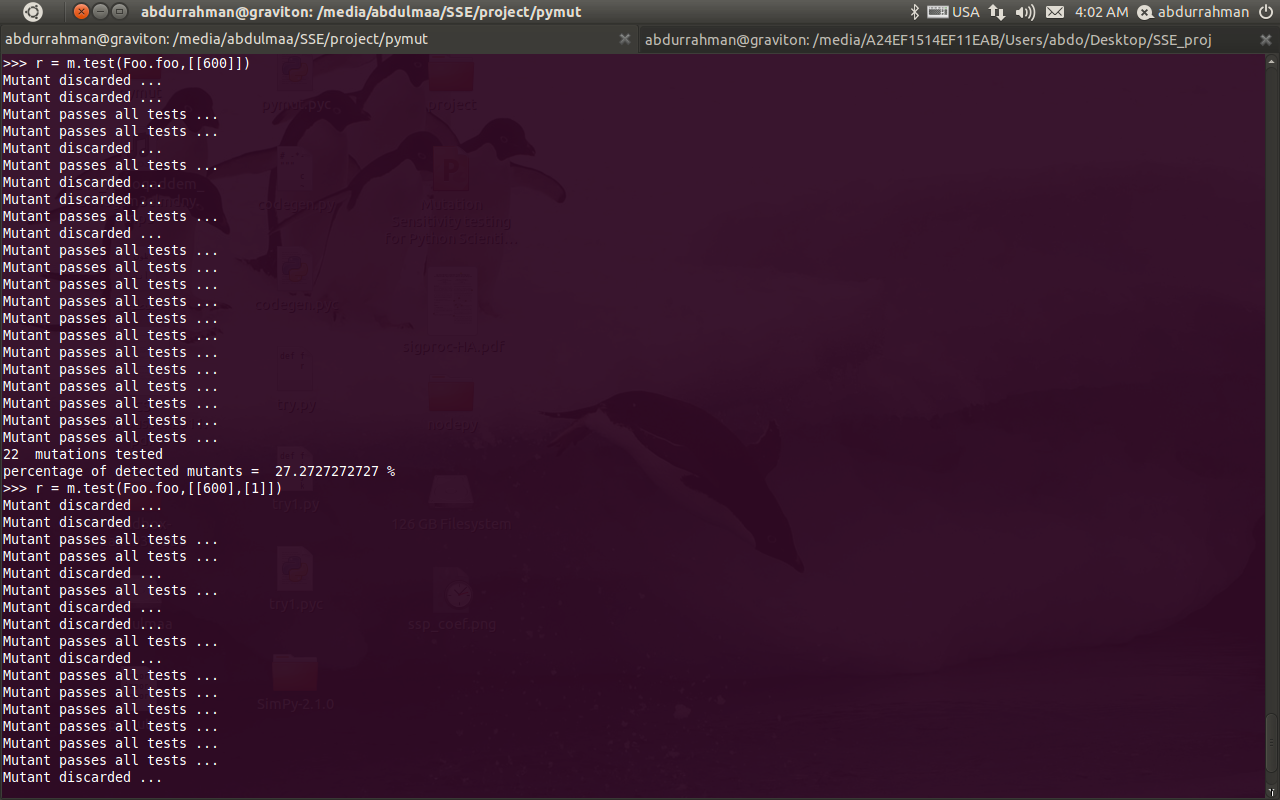
\includegraphics[trim = 0cm 11.3cm 25cm 1.9cm, clip, scale=0.4]{600.png}
\label{sh}
\end{figure}

In the second phase we used a python package called ``Nodepy'', or Numerical ODEs in Python (developed by D. Ketcheson at KAUST). Nodepy is around 2000 line of code. It is a package for designing, analysing, and testing numerical methods for initial value ODEs. Its development was motivated by the professor research in time integration methods for PDEs.\cite{a5}

As we started to test the package we realized that object oriented code may be harder to test. This is because usually some ``tasks'' need to be done (initialization of different objects) before the testing begins. Also we ound that mutating only the function that is to be tested is not practical. This is because it is usually the case that this function performs a small task, and depends on other functions. We thus added the ability to mutate more than one function while testing a single function. Figure ~\ref{ssp} shows the testing of a method in the Nodepy package.

\begin{figure}[h]
\caption{Testing Nodepy in the second phase}
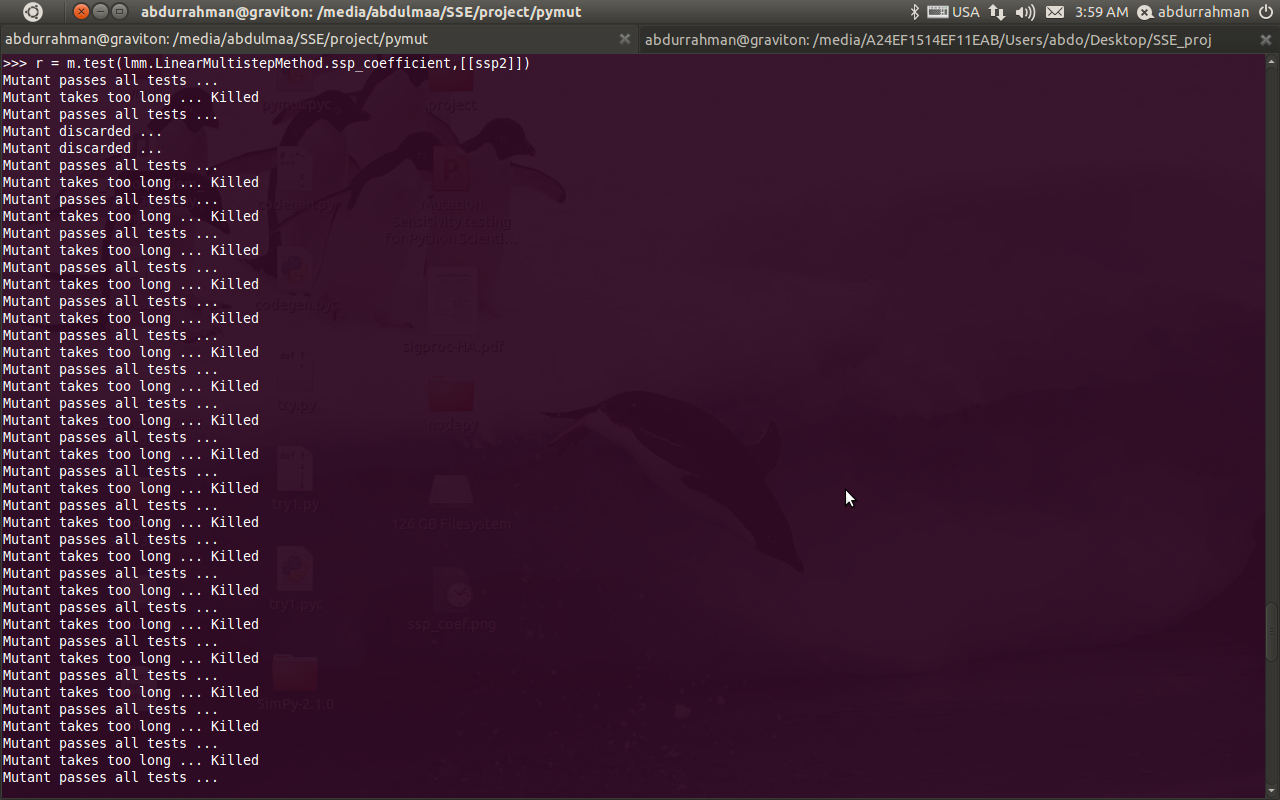
\includegraphics[trim = 0cm 14.9cm 25cm 1.9cm, clip, scale=0.4]{ssp_coef.png}
\label{ssp}
\end{figure}

\section{Using Pymut}

In this section we explain how Pymut should be used. Pymut is a python framework and can be used either within python code or using the interactive python interpreter.

To use Pymut, it should first be imported. This can be done as follows:
\begin{lstlisting}
>>> import Pymut as p
\end{lstlisting}

To use Pymut, a mutator object is needed. It can be created as follows:
\begin{lstlisting}
>>> m = p.Mutator(0.1,Mutator.relative,
 Mutator.high)
\end{lstlisting}

This creates a new Mutator object with a relative tolerance of 0.1 and high strictness (applies all test cases). The second two parameters for the constructor are optional and their default values are the ones used here. To use absolute tolerance, one can replace Mutator.relative with Mutator.absolute. Similarly one can replace Mutator.high with Mutator.medium or Mutator.low for a smaller number of mutation operators.

It is important to note here that Pymut works on function objects. To test a function, it must be sent to the mutator object as a function object. So assuming a function foo in the module Foo is to be tested, it should first be available:
\begin{lstlisting}
>>> import Foo
\end{lstlisting}

Assume foo takes as input one floating or int argument. A simple example that shows how foo can be tested with the arguments 1 and 2 is:
\begin{lstlisting}
>>> res = m.test(Foo.foo, [[1],[2]])
\end{lstlisting}

This will output a sequence of lines to the console that can be one of the following:

\begin{lstlisting}
Mutant takes too long ... Killed
Mutant passes all tests ...
Mutant discarded ...
\end{lstlisting}

A mutant is discarded if it fails one of the tests. The test function will return a list of mutants, here called `res'. This list contains only the mutants that passed all the tests. The user can then inspect these mutants to see if they are equivalent to the original code or not, and to add test cases that may fail them.

Assume however that the function foo calls another function foo\_helper that the used is also interested in mutating. That is to say, the user would only like to test foo, but they would like to test the effect of mutating foo\_helper on foo itself. A third (optional) argument can be passed to `test' that contains a list of function objects to be mutated along with the function that is being tested.

\begin{lstlisting}
>>> res = m.test(Foo.foo, [[1],[2]],
 [Foo.foo_helper])
\end{lstlisting}

It is important to point out that in python, the following two lines are equivalent regarding the instance method `ins\_method' of the object `someobj':

\begin{lstlisting}
>>> someobj.ins_method(param1, param2, ...)
>>> ins_method(someobj, param1, param2, ...)
\end{lstlisting}

This can thus be exploited to use Pymut to test instance methods as well as functions. Note however that, when testing instance methods, the method should be referenced by the class name, and not by the object name. For example, let someobj be an instance of SomeClass. The following is an incorrect way of testing ins\_method:

\begin{lstlisting}
>>> res = m.test(someobj.ins_method,
 [[someobj, param1, param2, ...]])
\end{lstlisting}

Instead, the following way of referencing ins\_method should be used:

\begin{lstlisting}
>>> res = m.test(SomeClass.ins_method, 
[[someobj, param1, param2, ...]])
\end{lstlisting}

\section{conclusion}

Mutation sensitivity testing is a software engineering tool that helps scientists to overcome the two big obstacles in testing their software: tolerance in comparing between results and the difficulties in having large number of oracles.

In this paper, we introduced a python framework for mutation testing that is suitable for scientists. It is a parse-based approach with extra added mutation types and operators. the presented framework gives the scientist the flexibility to choose the level of the test strictness and even the mutations to be applied. we also added to our framework a very helpful feature which gives the user some information about what test cases need to be added. Absolute sensitivity, relative sensitivity and traditional mutation testing are all implemented to give the scientist a range of testing options. 

With all mentioned, we emphasize that one of the problems that the mutation testing has is requiring a lot of space and time when generating the mutants for a large software. We tried to solve such a problem by introducing a less strict mutation testing which generates fewer number of mutants and produces reasonably reliable results. At the end, We run our framework on a scientific package written in python.

\section{Future Work}
Our platform can be implemented in other languages such as Java or/and C. Also, we need to dig more on how to overcome the problem of requiring a lot of space when running the test in large software.

\bibliographystyle{abbrv}
\bibliography{sigproc}  

\end{document}
